\vspace{-3pt}
\section{The Hadron Calorimeter}\label{sec:ch3:hcal}

\begin{figure}[h]
\centering
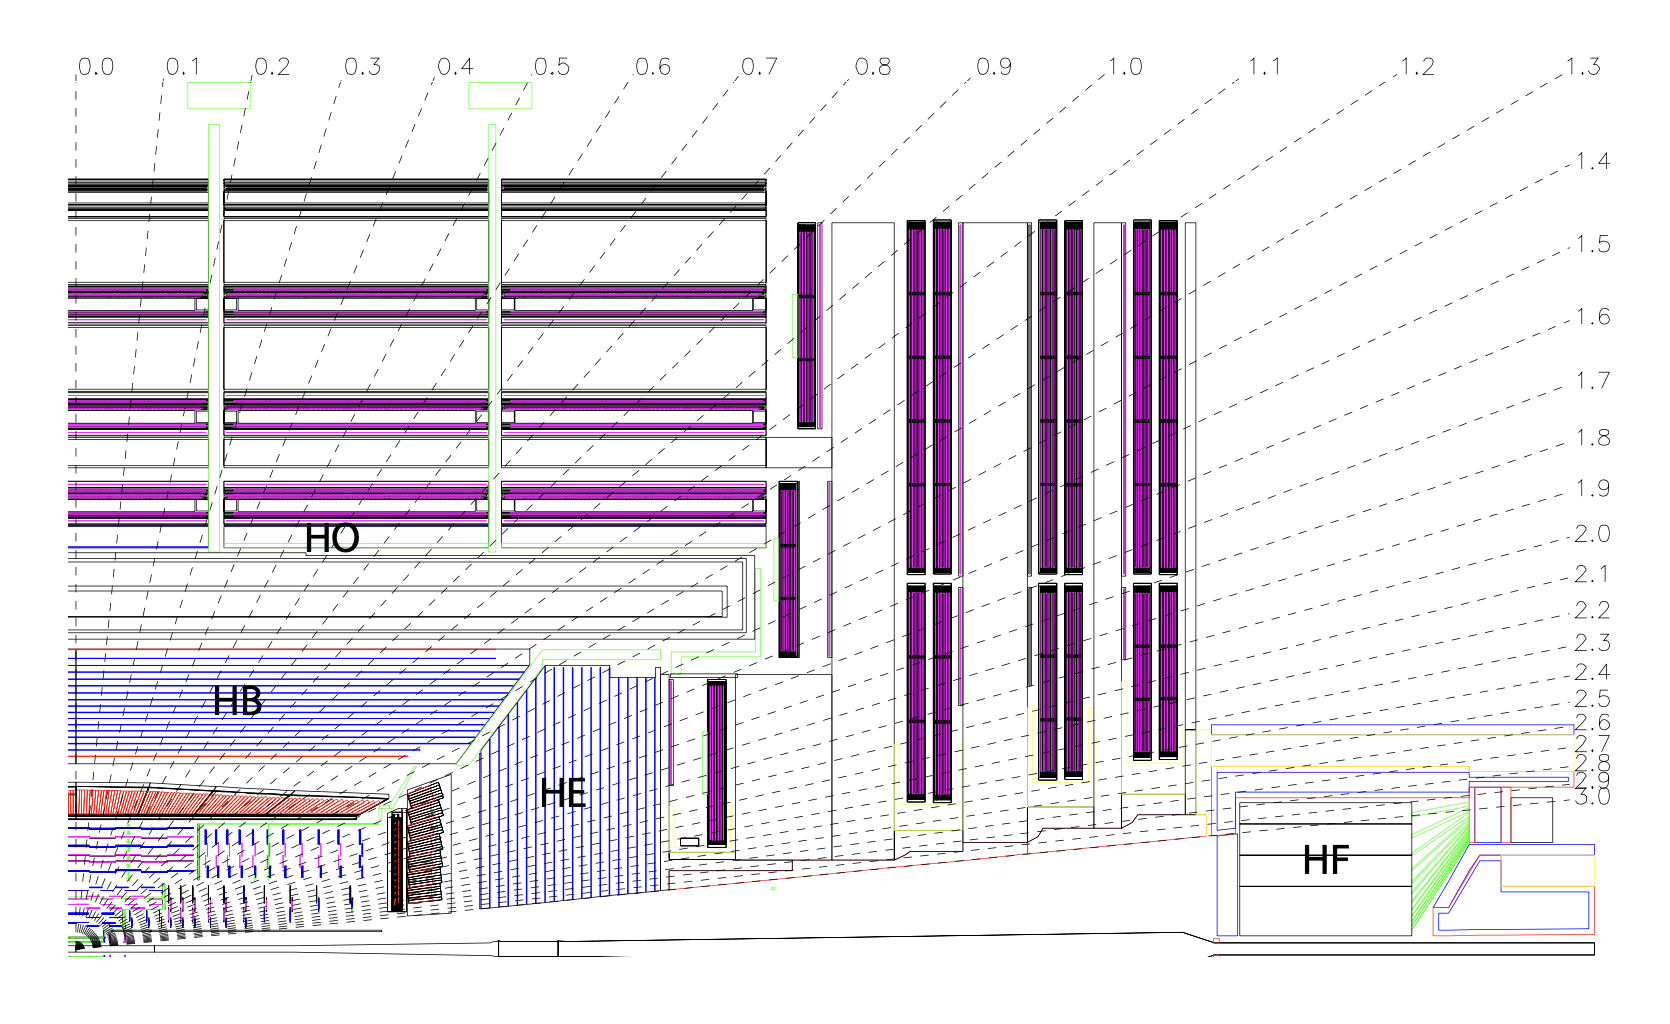
\includegraphics[width=1.0\textwidth]{figures/HCAL.png}
\caption{Schematic of the Hadron Calorimeter.}
\label{fig:HCAL}
\end{figure}


\begin{figure}[h]
\centering
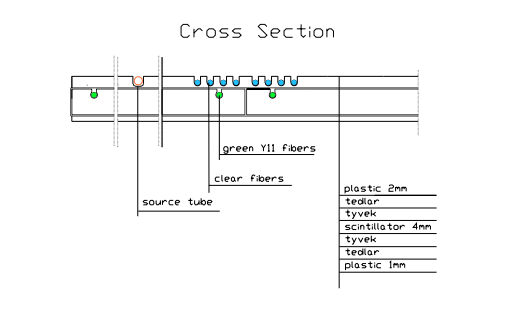
\includegraphics[width=1.0\textwidth]{figures/hcal_scintillator_replace.png}
\caption{Schematic of the plastic scintillator in the HCAL.}
\label{fig:HCAL_scint}
\end{figure}

The Hadron Calorimeter (HCAL) is designed to absorb the energy from the hadronic particles. It is split in four sections: the barrel (HB), the endcap (HE), the outer calorimeter (HO), and the forward calorimeter (HF), shown in Figure~\ref{fig:HCAL}. The barrel (HB), covers $|\eta| < 1.3$, and the endcaps (HE), cover $1.3 < |\eta| < 3.0$. The HB is a sampling calorimeter of absorber (bronze) and scintillator (plastic). The brass absorber is divided into 36 wedges in $\phi$. The plastic scintillator is divided into 16 sectors in $\eta$. The brass absorber is used for it's cost, radiation hardness, and non-magnetic properties.

The HCAL has a limited distance between the ECAL and the solenoid to absorb the hadronic particles. For particles that are unable to be stopped in that distance, an outer calorimeter is placed outside the solenoid in the central eta region



Hadrons penetrate more material than electrons and photons. Some hadrons still are not completely absorbed by the HCAL subdetectors between the ECAL and solenoid. Therefore the HO is set outside of the solenoid at R = 4.07 to catch any hadrons that are not stopped by the HB or HE. The HB is a sampling calorimeter with alternating layers of brass absorber and plastic scintillator. The brass absorber plates in the HB are positioned parallel to the beam line in a staggered formation. The first and last layer of the HB is a steel to serve as both an absorber layer and to provide structural strength. The HB has a total absorber length of 5.82 $\lambda_I$, where $\lambda_I$ is the interaction length of hadronic particles. The interaction length increases with $\theta$ as $1/\sin{\theta}$, for an thickness of 5.82 $\lambda_I$ at the edge of the HB at $|\eta| = 1.3$.

The scintillators are made of the material Kuraray SCSN81, which is a stable and radiation hard plastic. The plastic is formed into 70,000 tiles which are layered in trays between the brass absorber plates. One layer plastic scintillator sits in front of the steel absorber and one behind to catch any showers that start before the HCAL or that leak out the start of the HCAL. Tubes carry radioactive material through the plastic scintillator tiles for Cs$^{137}$ for calibration. A schematic of the plastic scintillator is shown in Figure~\ref{fig:HCAL_scint}.

The plastic scintillators detect the hadrons which are stopped by the brass absorbers. When a hadronic particle enters the plastic scintillator, the photoelectrons ionize and experience a gain of 2000 in the diode. Fiber optic cables in the scintillator carry the light to clear fiber. optic cables which carry the light to the photodiode. A diagram of a generic scintillator is shown in Figure~\ref{fig:scintillator}.

\begin{figure}[h]
\centering
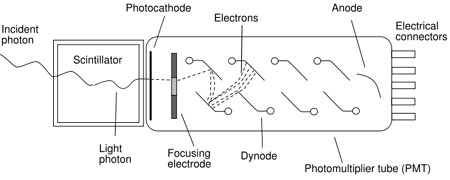
\includegraphics[width=1.0\textwidth]{figures/scintillator.jpg}
\caption{A scintillator converting an incoming photon to an electric signal.}
\label{fig:scintillator}
\end{figure}

The HB covers a pseudorapidity range of $|\eta| < 1.3$. The HE covers the range of $1.3 < |\eta| < 3$. The HE is also made of an alternating brass absorber and plastic scintillator. The HE covers 10 $\lambda_I$.

The solenoid also acts as an absorber with an interaction length of $1.4/\sin{\theta}$. Any hadrons that still have not been completely absorbed will then enter the outer HCAL (HO). With the HO, HB, and HE, the HCAL has a total absorption of 11.8 $\lambda_I$, with drops in efficiency only where the borders of the subdetectors meet.

The HF is made entirely of steel absorber with no scintillator between The HF is a thickness of 165 cm which corresponds to 10 $\lambda_I$ in steel. Electrons and photons will be absorbed within the first.